% =====================================================================
%  第 1 章 希尔伯特空间形式 —— ch01a（§1.1–§1.5）
%  页段：PDF 12–30（原书 p.11–29）
%  Lead 亲译的样板块：体例以此为准
% =====================================================================

\chapter{希尔伯特空间形式}

% [原文 p.11]
本章讲解量子力学的希尔伯特空间与算子进路的基本原理。这一形式体系以酉变换与测量为语言，为描述量子系统的演化建立了框架。

\section{状态空间}

\subsection{经典态}

经典力学与量子力学的一个根本差别，在于系统的态如何被描述。回忆经典力学中，粒子的态通常由相空间 $M$ 中的一个点来描述，$M$ 的几何由辛流形给出。在我们关心的大多数情形中，$M$ 由 $\{x_i,p_i\}$ 参数化：
\[
\begin{cases}
x_i=\text{（广义）位置},\\
p_i=\text{与 } x_i \text{ 共轭的（广义）动量}.
\end{cases}
\]
态的随时间演化由以时间为参数的轨道描述：
\[
\{x_i(t),p_i(t)\}:\quad \text{时刻 } t \text{ 的态}.
\]
在哈密顿形式中，这一经典演化由\emph{哈密顿方程}（Hamilton's equations）描述
\[
\begin{cases}
\dfrac{\rd x_i}{\rd t}=\dfrac{\pa H}{\pa p_i},\\[3mm]
\dfrac{\rd p_i}{\rd t}=-\dfrac{\pa H}{\pa x_i}.
\end{cases}
\]
这里 $H$ 是相空间上的函数，称为\emph{哈密顿函数}。哈密顿方程组决定了态的演化。

\subsection{量子态}

量子力学中，粒子的态由希尔伯特空间 $V$ 中的一个向量表示。我们始终假定希尔伯特空间 $V$ 是可分的。

\begin{definition}{1.1.1}
  \textbf{希尔伯特空间}（Hilbert space）是指带有一个正定厄米内积的 $\C$ 线性向量空间，并且该空间关于内积诱导的范数完备。
\end{definition}

% [原文 p.12]
也可以谈论 $\R$ 线性希尔伯特空间，但我们聚焦于 $\C$ 线性的情形。我们将会看到，角相位因子在量子力学中起着重要作用。

设 $V$ 是希尔伯特空间。厄米内积是一个半双线性配对
\[
\langle-|-\rangle:V\times V\longrightarrow\C,
\]
它对第一个变元共轭线性、对第二个变元线性：
\[
\begin{cases}
\langle\lambda\psi|\phi\rangle=\overline{\lambda}\,\langle\psi|\phi\rangle,\\
\langle\psi|\lambda\phi\rangle=\lambda\langle\psi|\phi\rangle,
\end{cases}
\qquad \forall\lambda\in\C,\ \psi,\phi\in V.
\]
厄米性说的是
\[
\langle\psi|\phi\rangle=\overline{\langle\phi|\psi\rangle},
\qquad \forall\psi,\phi\in V.
\]
正定性说的是
\[
\begin{cases}
\langle\psi|\psi\rangle\ge 0,&\forall\psi\in V,\\
\langle\psi|\psi\rangle=0&\Longleftrightarrow\ \psi=0.
\end{cases}
\]
$V$ 上诱导的范数由
\[
\norm{\psi}:=\sqrt{\langle\psi|\psi\rangle},\qquad \psi\in V
\]
给出。作为希尔伯特空间，$V$ 必须关于范数 $\norm{\cdot}$ 完备。

\begin{example}{1.1.2}
  $V=\C^n$。向量 $u\in V$ 表示为
  \[
  u=\begin{pmatrix}z_1\\ \vdots\\ z_n\end{pmatrix},\qquad z_i\in\C.
  \]
  我们可用
  \[
  \langle u|v\rangle=\sum_i \bar z_i w_i
  \]
  定义标准厄米内积，其中 $u=(z_1\ \cdots\ z_n)^T$，$v=(w_1\ \cdots\ w_n)^T$。于是 $\C^n$ 是有限维希尔伯特空间。
\end{example}

\begin{example}{1.1.3}
  $V=L^2(\R)$。对任意 $f,g\in L^2(\R)$，定义
  \[
  \langle f|g\rangle=\int_\R \overline{f(x)}\,g(x)\,\rd x.
  \]
  这给出一个无穷维希尔伯特空间。
\end{example}

\begin{remark}{1.1.4}
  我们将使用狄拉克的左右矢记号，把向量 $\psi\in V$ 写成“右矢”（ket）$\ket{\psi}\in V$。
\end{remark}

% [原文 p.13]
$\phi\in V$ 的“左矢”（bra）$\bra{\phi}$ 表示线性形式
\[
\bra{\phi}:V\longrightarrow\C,\qquad \ket{\psi}\longmapsto \braket{\phi}{\psi}.
\]
换言之，“左矢”与“右矢”之间以厄米共轭相联系。以 $V=\C^n$ 为例，给定
\[
u=\begin{pmatrix}z_1\\ \vdots\\ z_n\end{pmatrix},\qquad
v=\begin{pmatrix}w_1\\ \vdots\\ w_n\end{pmatrix}\in V,
\]
我们可以表示
\begin{enumerate}[label=(\arabic*),leftmargin=3.2em,itemsep=1pt]
  \item “右矢”：$\ket{v}=\begin{pmatrix}w_1\\ \vdots\\ w_n\end{pmatrix}$；
  \item “左矢”：$\bra{u}=(\bar z_1\ \cdots\ \bar z_n)$。
\end{enumerate}
于是厄米内积是
\[
\braket{u}{v}=(\bar z_1\ \cdots\ \bar z_n)\cdot
\begin{pmatrix}w_1\\ \vdots\\ w_n\end{pmatrix}.
\]

那么，从经典到量子，对态的描述发生的本质变化是什么？

\begin{center}
\begin{tabular}{c c}
\toprule
经典态 & 量子态\\
\midrule
集合 & 向量空间\\
\bottomrule
\end{tabular}
\end{center}

态空间的代数结构已由“集合”加强为“向量空间”！这特别意味着，我们可以把两个量子态 $\ket{\psi_1},\ket{\psi_2}\in V$ 作线性叠加，得到另一个量子态
\[
\lambda_1\ket{\psi_1}+\lambda_2\ket{\psi_2}\in V,
\]
其中 $\lambda_1,\lambda_2\in\C$。这种线性运算在经典态的集合上是不允许的。后文将会看到，许多有趣的量子现象正来源于这一线性结构。

为获得初步印象，考虑一个由二维希尔伯特空间描述的量子系统，该空间由
\[
\ket{\uparrow},\qquad \ket{\downarrow}
\]
张成。例如，这可以是一个自旋系统，其中 $\ket{\uparrow}$ 表示“自旋向上”的态，$\ket{\downarrow}$ 表示“自旋向下”的态。于是我们可以作组合，得到态
\[
\frac{1}{\sqrt2}\ket{\uparrow}+\frac{1}{\sqrt2}\ket{\downarrow}.
\]
这是一个新的态。但它的自旋是什么？阅读本书时，请把这个简单的问题记在心里。它与 $\ket{\uparrow}$ 或 $\ket{\downarrow}$ 同样是合法的态。

% [原文 p.14]
作为说明性的另一个例子，我们考虑如何描述两个粒子的态。经典情形下，若第 $i$ 个粒子的态集合为 $M_i$（$i=1,2$），则整体的态空间是
\[
M_1\times M_2.
\]
量子情形下，若第 $i$ 个粒子的态空间为 $V_i$，则朴素的集合论乘积 $V_1\times V_2$ 行不通，原因很简单：$V_1\times V_2$ 不是线性向量空间。我们只能考虑它的线性化，由此得到张量积
\[
V_1\otimes V_2.
\]
$M_1\times M_2$ 与 $V_1\otimes V_2$ 的一个关键差别在于：$M_1\times M_2$ 中的点是
\[
m_1\times m_2,\qquad m_1\in M_1,\ m_2\in M_2
\]
这种形状，而 $V_1\otimes V_2$ 中的向量可以是
\[
\sum_{i=1}^{k}\psi_i\otimes\phi_i,\qquad \psi_i\in V_1,\ \phi_i\in V_2
\]
这种形状。例如，这一张量结构正是量子纠缠的起源。

\takeaway{本节把“态”从相空间中的一个点换成希尔伯特空间中的一个向量：经典演化是哈密顿方程给出的轨道，量子演化是薛定谔方程给出的酉变换；叠加原理与张量积由此进入，后者正是纠缠的代数来源。}

\subsection{薛定谔方程}

接下来讨论支配量子态随时间演化的规律。

\begin{definition}{1.1.5}
  设 $A$ 是希尔伯特空间 $V$ 上的线性算子，其定义域 $\Dom(A)\subset V$ 稠密。$A$ 的\emph{伴随算子}（adjoint operator）$A^*$ 定义为
  \[
  A^*:\Dom(A^*)\longrightarrow V,
  \]
  其中 $A^*$ 的定义域是
  \[
  \Dom(A^*)=\Bigl\{\psi\in V\ \Big|\ \exists\,\tilde\psi\in V:\ 
  \langle\psi|A\phi\rangle=\langle\tilde\psi|\phi\rangle,\ \forall\phi\in\Dom(A)\Bigr\}.
  \]
  这里，对 $\psi\in\Dom(A^*)$ 及如上所述的 $\tilde\psi$，令
  \[
  A^*\psi=\tilde\psi.
  \]
  象征地写，伴随算子的定义关系是
  \[
  \langle A^*\psi|\phi\rangle=\langle\psi|A\phi\rangle,
  \qquad \phi\in\Dom(A),\ \psi\in\Dom(A^*).
  \]
\end{definition}

\begin{definition}{1.1.6}
  若 $A=A^*$，则称 $A$ 是\emph{自伴的}（self-adjoint）。
\end{definition}

% [原文 p.15]
\begin{remark}{1.1.7}
  当 $V$ 有限维、$A$ 由矩阵表示时，$A^*$ 由共轭转置给出。此时自伴算子与厄米矩阵是一回事。当 $V$ 无穷维时——这正是量子力学所关心的情形——自伴算子要微妙得多，我们必须与稠密定义的定义域打交道。关于希尔伯特空间上的自伴算子，系统的讨论见 §4.1。
\end{remark}

量子力学中，量子态 $\ket{\psi(t)}$ 的随时间演化服从\emph{薛定谔方程}（Schrödinger equation）：
\[
\ii\hbar\frac{\rd}{\rd t}\ket{\psi(t)}=\hat H\ket{\psi(t)}.
\]
这里 $\hat H$ 是自伴算子，称为\emph{哈密顿算子}。正数 $\hbar$ 称为\emph{普朗克常数}，是物理学的基本常数之一。

设 $\hat H$ 不依赖时间，则薛定谔方程可形式地解为
\[
\ket{\psi(t)}=\ee^{-\ii\hat H t/\hbar}\ket{\psi(0)}.
\]
算子 $\ee^{-\ii\hat H t/\hbar}$（可用泛函演算定义）是 $V$ 上单参数族的酉算子，称为\emph{时间演化算子}。反过来，强连续的单参数酉变换族由某个自伴算子无穷小地生成，这就是\emph{斯通定理}（Stone's Theorem，见 §4.3）。

\section{可观测量}

\subsection{经典可观测量}

经典力学中，可观测量由相空间 $M$ 上的函数表示：
\[
\mathrm{Obs}_{\mathrm{cl}}=\mathcal{O}(M).
\]
这里 $\mathcal{O}(M)$ 指 $M$ 上（适当的）函数空间。我们不具体指定函数类，以免陷入与目的无关的技术讨论；在这里，放心地用光滑函数即可。

由于 $M$ 是辛流形，其上的函数空间 $\mathcal{O}(M)$ 自然带有泊松括号的结构
\[
\{-,-\}:\mathcal{O}(M)\times\mathcal{O}(M)\longrightarrow\mathcal{O}(M).
\]
它是双线性映射，并满足下述性质：
\begin{itemize}[leftmargin=2em,itemsep=1pt]
  \item 反对称性：$\{f,g\}=-\{g,f\}$。
  \item 莱布尼茨律：$\{f,gh\}=\{f,g\}h+g\{f,h\}$。
  \item 雅可比恒等式：$\{\{f,g\},h\}+\{\{g,h\},f\}+\{\{h,f\},g\}=0$。
\end{itemize}

% [原文 p.16]
例如，设相空间 $M$ 由 $\{x_i\}$ 及其共轭 $\{p_i\}$ 参数化，使得辛结构取形状
\[
\sum_i \rd x_i\wedge \rd p_i.
\]
则经典可观测量是 $\{x_i,p_i\}$ 的函数 $f(x,p)$，而泊松括号取形状
\[
\{f,g\}=\sum_i\left(\frac{\pa f}{\pa x_i}\frac{\pa g}{\pa p_i}-\frac{\pa f}{\pa p_i}\frac{\pa g}{\pa x_i}\right).
\]

\subsection{量子可观测量}

量子力学中，量子可观测量由系统希尔伯特空间 $V$ 上的自伴线性算子构成。我们已经见过一个这样的量子可观测量，即哈密顿算子 $\hat H$，它通过薛定谔方程支配系统的动力学演化。

记 $\mathrm{Obs}_{\mathrm{q}}$ 为量子可观测量的空间。设 $A,B$ 是两个自伴算子
\[
A=A^*,\qquad B=B^*.
\]
考虑它们的\emph{交换子}（commutator）
\[
[A,B]:=AB-BA.
\]
其伴随为
\[
[A,B]^*=B^*A^*-A^*B^*=[B^*,A^*]=[B,A]=-[A,B].
\]
因此 $\ii[A,B]$ 仍是自伴的。组合
\[
[-,-]_{\hbar}:=-\frac{\ii}{\hbar}[-,-]:\mathrm{Obs}_{\mathrm{q}}\times\mathrm{Obs}_{\mathrm{q}}\longrightarrow\mathrm{Obs}_{\mathrm{q}}
\]
定义了量子可观测量上的\emph{量子括号}。这里正数 $\hbar$ 是普朗克常数。量子括号仍是反对称的
\[
[A,B]_{\hbar}=-[B,A]_{\hbar},
\]
并满足雅可比恒等式
\[
[A,[B,C]_{\hbar}]_{\hbar}+[B,[C,A]_{\hbar}]_{\hbar}+[C,[A,B]_{\hbar}]_{\hbar}=0.
\]
这些性质来自算子复合的结合性。

经典可观测量与量子可观测量之间的代数关系可概述为

\begin{center}
\begin{tabular}{ccc}
\toprule
$\mathrm{Obs}_{\mathrm{cl}}$ & & $\mathrm{Obs}_{\mathrm{q}}$\\
\midrule
泊松代数 & $\xrightarrow{\ \text{量子化}\ }$ & 结合代数\\
$(\cdot,\{-,-\})$ & $\xleftarrow{\ \text{经典极限}\ }$ & $(*_{\hbar},[-,-]_{\hbar})$\\
\bottomrule
\end{tabular}
\end{center}

% [原文 p.17]
经典泊松括号 $\{-,-\}$ 度量了量子算子的首阶非交换性。严格地说，为了作复合、构成结合代数，我们把 $\mathrm{Obs}_{\mathrm{q}}$ 扩张为包含非自伴线性算子。研究这种代数对应，正是形变量子化的主题，我们将在第 6 章详细讨论。

\subsection{期望}

设 $V$ 是量子系统的希尔伯特空间。设 $O$ 是一个量子可观测量，即 $V$ 上的自伴算子。设系统处于态 $\ket{\psi}\in V$。系统关于 $O$ 的\emph{期望值}（expectation value）定义为
\[
\expv{O}_{\psi}:=\frac{\braket{\psi}{O|\psi}}{\braket{\psi}{\psi}}.
\]
这里 $O\ket{\psi}=\ket{O\psi}$ 是 $O$ 对态 $\ket{\psi}$ 的作用。把态归一化，使得
\[
\norm{\psi}=\sqrt{\braket{\psi}{\psi}}=1,
\]
会很方便。许多场合下，量子系统的态就指希尔伯特空间中的归一向量；于是在归一化的情形
\[
\expv{O}_{\psi}=\braket{\psi}{O|\psi}.
\]
注意量子可观测量的期望值是实数。事实上，
\[
\braket{\psi}{O|\psi}=\braket{\psi}{O\psi}
=\braket{O^*\psi}{\psi}
\overset{O^*=O}{=}\braket{O\psi}{\psi}
=\overline{\braket{\psi}{O\psi}}
=\overline{\braket{\psi}{O|\psi}},
\]
故 $\expv{O}_{\psi}\in\R$。这里我们用了 $O$ 的自伴性。这说明 $O$ 的本征值是实数。

设 $\ket{\psi}$ 是 $A$ 的归一本征向量，本征值为 $\lambda$。按上面的讨论，$\lambda$ 必为实数。稍后我们会看到，本征值正是量子可观测量物理测量的结果。

\takeaway{本节把可观测量从“相空间上的函数加泊松括号”换成“希尔伯特空间上的自伴算子加交换子”：自伴性保证期望与本征值都是实数，而 $\hbar\to0$ 时量子括号退化为泊松括号。}

\section{测量}

\subsection{玻恩规则}

前面已经讨论了量子力学的两条基本公设：
\begin{itemize}[leftmargin=2em,itemsep=1pt]
  \item 量子态是希尔伯特空间 $V$ 中的一个向量；
  \item 量子可观测量是 $V$ 上的自伴算子。
\end{itemize}
下面转向对给定量子态下量子可观测量的测量作诠释。第一条论断是

% [原文 p.18]
\begin{itemize}[leftmargin=2em,itemsep=1pt]
  \item 量子测量的可能结果，是量子可观测量的本征值。
\end{itemize}
设 $O$ 是量子可观测量，即 $V$ 上的自伴算子。如上所见，自伴性意味着 $O$ 的本征值全为实数。上述公设说，这些实数就是测量 $O$ 的可能结果。

设系统现在处于态 $\ket{\psi}\in V$。那么，在一次测量中，如何从量子态 $\ket{\psi}$ 得到 $O$ 的一个本征值？

首先，设 $\ket{\psi}$ 是 $O$ 的本征向量，本征值为 $\lambda$：
\[
O\ket{\psi}=\lambda\ket{\psi}.
\]
那么自然会期望，在态 $\ket{\psi}$ 中测量 $O$ 的结果是 $\lambda$。事实确实如此。但一般而言 $\ket{\psi}$ 未必是 $O$ 的本征向量，这时我们得到什么？答案是概率性的，称为\emph{玻恩规则}（Born rule）。

先说明一点：$V$ 中相差一个非零复数的两个向量，表示同一个物理态。换言之，每个物理态由希尔伯特空间 $V$ 中的一条“射线”表示。例如，量子可观测量 $O$ 在态 $\ket{\psi}$ 中的期望值
\[
\expv{O}_{\psi}=\frac{\braket{\psi}{O|\psi}}{\braket{\psi}{\psi}}
\]
在你把 $\ket{\psi}$ 换为 $a\ket{\psi}$（$a\in\C^*$）后不变。因此我们通常把态归一化，用长度为 $1$ 的向量表示物理态
\[
\braket{\psi}{\psi}=1.
\]
我们称这种单位长度的向量为\emph{归一态}。

设 $O$ 是给定的量子可观测量。设 $\ket{\psi_1}$ 与 $\ket{\psi_2}$ 是本征向量
\[
O\ket{\psi_1}=\lambda_1\ket{\psi_1},\qquad O\ket{\psi_2}=\lambda_2\ket{\psi_2},
\]
本征值不同，$\lambda_1\ne\lambda_2$。则这两个向量 $\ket{\psi_1}$ 与 $\ket{\psi_2}$ 必定正交：
\[
\braket{\psi_1}{\psi_2}=0.
\]
这由 $O$ 的自伴性推出：
\[
\lambda_2\braket{\psi_1}{\psi_2}=\braket{\psi_1}{O\psi_2}
=\braket{O\psi_1}{\psi_2}=\lambda_1\braket{\psi_1}{\psi_2}
\ \Longrightarrow\ \braket{\psi_1}{\psi_2}=0.
\]
若 $\ket{\psi_1}$ 与 $\ket{\psi_2}$ 有相同本征值 $\lambda_1=\lambda_2$，则它们未必正交；不过我们可以用格拉姆–施密特（Gram–Schmidt）步骤把它们重新安排为正交。

设被测量的系统的量子态 $\ket{\psi}$ 可按量子可观测量 $O$ 的正交归一本征态分解
\[
\ket{\psi}=\sum_{\alpha}c_{\alpha}\ket{\psi_{\alpha}},\qquad c_{\alpha}\in\C.
\]

% [原文 p.19]
这里 $O\ket{\psi_{\alpha}}=\lambda_{\alpha}\ket{\psi_{\alpha}}$，$\lambda_{\alpha}$ 为本征值，而 $\ket{\psi_{\alpha}}$ 是归一向量，不同 $\alpha$ 之间彼此正交。当某些 $\lambda_{\alpha}$ 相同时（即本征子空间简并），或本征值谱连续时（例子见 §1.8），情形可能更复杂。此刻我们不必顾虑这些问题。

设 $\ket{\psi}$ 是归一的。归一化条件 $\braket{\psi}{\psi}=1$ 结合 $\ket{\psi_{\alpha}}$ 的正交归一性，给出
\[
\sum_{\alpha}\abs{c_{\alpha}}^2=1.
\]
人们把这个式子诠释为概率。

\textbf{玻恩规则}：在量子态 $\ket{\psi}$ 中测量量子可观测量 $O$，其结果具有概率性：测得答案 $\lambda$ 的概率是
\[
P(\lambda)=\sum_{\lambda_{\alpha}=\lambda}\abs{c_{\alpha}}^2.
\]
利用正交归一性，复数 $c_{\alpha}$ 可由
\[
c_{\alpha}=\braket{\psi_{\alpha}}{\psi}
\]
得到，$c_{\alpha}$ 称为\emph{概率振幅}。于是玻恩规则可表述为
\[
\text{概率}=\abs{\text{振幅}}^2.
\]

\begin{remark}{1.3.1}
  这一概率分布的精确数学构造，就是 §4.2.3 所述的谱测度概念。
\end{remark}

\subsection{态向量的塌缩}

量子力学中的测量实验本质上涉及复合系统。换一种说法：对量子系统的任何测量（借助外部仪器）都会扰动该态。事实上，情况还要更神秘：在测量量子可观测量 $O$ 并得到本征值 $\lambda$ 之后，态会变成与本征值 $\lambda$ 相应的本征态。这一现象称为\emph{“态向量的塌缩”}（collapse of the state vector）。由于测量之后态成为本征向量，若系统不再受其他扰动，则对 $O$ 的进一步重复测量将总是给出 $\lambda$。

关于量子力学的含义，包括上述玻恩规则与态向量塌缩，有一整套看法，形成了“哥本哈根诠释”这一名目。它并不完全令人满意，在历史上引出了许多困惑与争论。关于塌缩，还有休·埃弗里特（Hugh Everett）的“多世界诠释”：它假定态向量并不塌缩，而是量子测量的一切可能结果都在某些平行世界中实现。我们在此不再深入这些问题。

尽管如此，量子力学是有效的，并且是物理学中最成功的框架之一。许多人持实用的观点。下面是戴维·默明（David Mermin）的一句名言：

% [原文 p.20]
\begin{quote}
“如果我被迫用一句话概括哥本哈根诠释对我说了什么，那就是：\emph{‘闭嘴，去计算！’}”
\end{quote}
{\small （原话：“If I were forced to sum up in one sentence what the Copenhagen interpretation says to me, it would be ‘Shut up and calculate!’”）\par}

于是我们看到：虽然态的演化是确定性的、由薛定谔方程刻画，但对测量的预言却是概率性的；不仅如此，测量还会改变态。那么我们如何检验量子力学？

要检验这种概率性预言，我们需要制备一个量子系综，由大量处于同一态的粒子组成；然后对每个粒子作同样的测量。每次测量的结果都以某个本征值为终结，而对同态中另一个粒子的重复测量，结果可能不同。于是我们可以收集这些测量的统计结果，与概率性预言相对照。

\subsection{双缝实验}

考虑如下实验装置：左边有一个源 $S$，能向各方向发射粒子；中间有一堵墙，上面开两个小孔；右边有一个屏，它是一个探测器，能在每个粒子到达时记录下来。

\begin{center}
\begin{tikzpicture}[scale=0.95,>=Stealth]
  % 源
  \fill (0,0) circle (2pt);
  \node[below,yshift=-1pt] at (0,0) {\small $S$};
  \foreach \a in {22,0,-22}{\draw[->] (0.12,0) -- ++(\a:0.95);}
  % 墙
  \draw[thick] (3.4,1.7) -- (3.4,0.42);
  \draw[thick] (3.4,0.16) -- (3.4,-0.16);
  \draw[thick] (3.4,-0.42) -- (3.4,-1.7);
  \node[right] at (3.5,0.95) {\small 1};
  \node[right] at (3.5,-0.95) {\small 2};
  % 屏
  \draw[thick] (6.0,1.7) -- (6.0,-1.7);
  % 标注
  \node[below] at (0,-1.95) {\small 源};
  \node[below] at (3.4,-1.95) {\small 墙};
  \node[below] at (6.0,-1.95) {\small 探测器};
\end{tikzpicture}
\end{center}

% [图：原书 p.20，本图按原文重绘，图内标注已译为中文；原图无题注]

我们要找的是探测器上粒子计数的结果分布。

在经典图像中，若把小孔 2 堵上，我们在探测器上得到一个粒子计数分布，它们只来自小孔 1，记之为 $P_1$。同样，若堵上小孔 1、留着孔 2，我们得到只计来自孔 2 的粒子的分布 $P_2$。现在若两孔都打开，我们将看到探测器上的分布是上述两个分布之和
\[
P=P_1+P_2.
\]
所得的分布 $P$ 会像

\begin{center}
\begin{tikzpicture}[scale=0.95,>=Stealth]
  % 墙
  \draw[thick] (0,1.55) -- (0,0.55);
  \draw[thick] (0,0.35) -- (0,-0.35);
  \draw[thick] (0,-0.55) -- (0,-1.55);
  \node[left] at (-0.15,0.95) {\small 1};
  \node[left] at (-0.15,-0.95) {\small 2};
  % 屏 + 分布曲线
  \draw[thick] (3.2,1.55) -- (3.2,-1.55);
  \draw[blue,thick] plot[domain=-1.5:1.5,samples=60]
     ({3.2+0.85*exp(-2.2*\x*\x)},{ \x});
  \node[blue] at (4.35,1.35) {\small $P$};
  % 射线
  \draw[->] (0.05,0.95) -- (3.1,0.12);
  \draw[->] (0.05,-0.95) -- (3.1,-0.12);
  % 标注
  \node[below] at (0,-1.8) {\small 墙};
  \node[below] at (3.2,-1.8) {\small 探测器};
  \node[left] at (-1.75,0) {\small\underline{经典图像}：};
\end{tikzpicture}
\end{center}

% [图：原书 p.20，按原文重绘]

% [原文 p.21]
量子情形下，上述两种情形的叠加。由线性关系
\[
\braket{\phi}{\psi_1+\psi_2}=\braket{\phi}{\psi_1}+\braket{\phi}{\psi_2}
\]
可见，被求和的是各情形下的概率振幅
\[
A=A_1+A_2.
\]
如我们所见，测量的概率分布是振幅的平方
\[
P_1=\abs{A_1}^2,\qquad P_2=\abs{A_2}^2,\qquad P=\abs{A}^2=\abs{A_1+A_2}^2.
\]
由于振幅是复数，
\[
P\ne P_1+P_2,
\]
我们将观察到像光波那样的干涉图样。

\begin{center}
\begin{tikzpicture}[scale=0.95,>=Stealth]
  % 墙
  \draw[thick] (0,1.55) -- (0,0.55);
  \draw[thick] (0,0.35) -- (0,-0.35);
  \draw[thick] (0,-0.55) -- (0,-1.55);
  \node[left] at (-0.15,0.95) {\small 1};
  \node[left] at (-0.15,-0.95) {\small 2};
  % 屏 + 干涉图样
  \draw[thick] (3.2,1.55) -- (3.2,-1.55);
  \draw[blue,thick] plot[domain=-1.5:1.5,samples=200]
     ({3.2+0.85*exp(-0.9*\x*\x)*(1+0.75*cos(9*\x r))},{ \x});
  \node[blue] at (4.65,1.35) {\small $P$};
  % 两孔向右发出的球面波前（同心圆弧）
  \foreach \r in {0.5,0.85,1.2}{
    \draw[red] (0,0.95) arc (-55:55:\r);
    \draw[red] (0,-0.95) arc (-55:55:\r);
  }
  \node[below] at (0,-1.8) {\small 墙};
  \node[below] at (3.2,-1.8) {\small 探测器};
  \node[left] at (-1.75,0) {\small\underline{量子图像}：};
\end{tikzpicture}
\end{center}

% [图：原书 p.21，按原文重绘]

这可以用一束量子粒子（比如电子）来检验。结果确实显示出量子图像的干涉图样。

这令人惊讶。人们可能试图在狭缝附近放置探测装置，以判断每个粒子经过哪条缝。要作这种测量，你必然扰动粒子的态。例如，你可以用光子在小孔处探测电子。这样的测量会使态向量塌缩，结果你会发现干涉图样消失，回到经典图像。量子粒子同时表现出波与粒子的行为！这就是\emph{波粒二象性}的概念。

双缝实验最初是为演示\emph{光}的波动行为而设计的。是德布罗意（de Broglie）勇敢地提出假设：一切物质都具有波动性质。这一预言很快在电子上得到验证。

\takeaway{本节给出量子力学的第三条公设：测量结果为可观测量的本征值，概率由玻恩规则“概率 = 振幅的模方”给出，测量之后态塌缩到相应本征态；双缝实验把这套概率规则表现为干涉图样。}

\section{不确定原理}

\subsection{交换子与不确定性}

对量子可观测量 $O$ 的测量将给出 $O$ 的一个本征值，并使态塌缩为 $O$ 的一个本征向量。人们自然会问：能否同时测量两个量子可观测量？例如，我们希望同时测量位置与动量。这在经典力学中不成问题；但在量子力学中，我们就会遇到麻烦。

设 $A,B$ 是两个量子可观测量。我们关于测量的公设要求：在一并测量它们时，要取 $A$ 与 $B$ 的公共本征向量。而如线性代数中所学，若 $A$ 与 $B$ 不交换，公共本征向量可能不存在。例如，设 $A$ 与 $B$ 满足
\[
[A,B]=\ii I,
\]
其中 $I$ 是恒等算子。设 $\ket{\psi}$ 是 $A$ 与 $B$ 的公共本征向量，
\[
A\ket{\psi}=\lambda_1\ket{\psi},\qquad B\ket{\psi}=\lambda_2\ket{\psi}.
\]
则
\[
\ii\ket{\psi}=[A,B]\ket{\psi}=(AB-BA)\ket{\psi}
=(\lambda_1\lambda_2-\lambda_2\lambda_1)\ket{\psi}=0.
\]
于是同时测量的问题与量子可观测量的交换子有关。我们首先引入量子可观测量在给定态中的不确定性这一概念。

\begin{definition}{1.4.1}
  可观测量 $O$ 在量子态 $\ket{\psi}$ 中的\emph{不确定性}定义为
  \[
  (\Delta_{\psi}O)^2:=\bigl\langle (O-\expv{O}_{\psi})^2\bigr\rangle_{\psi}.
  \]
\end{definition}

% [原文 p.22]
具体写出：设 $\ket{\psi}$ 是归一态。由于 $\expv{O}_{\psi}\in\R$，有
\[
(\Delta_{\psi}O)^2
=\bigl\langle (O-\expv{O}_{\psi})\psi\,\big|\,(O-\expv{O}_{\psi})\psi\bigr\rangle.
\]
特别地，$\Delta_{\psi}O=0$ 当且仅当
\[
O\ket{\psi}=\expv{O}_{\psi}\ket{\psi},
\]
即当且仅当 $\ket{\psi}$ 是 $O$ 的本征向量。此时对 $O$ 的测量是确定的，结果就是相应的本征值。一般地，不确定性度量的是围绕期望的平均涨落。在概率论中，不确定性也称为\emph{标准差}。注意我们还有
\[
(\Delta_{\psi}O)^2
=\bigl\langle O^2-2\expv{O}_{\psi}O+\expv{O}_{\psi}^2\bigr\rangle_{\psi}
=\expv{O^2}_{\psi}-\expv{O}_{\psi}^2.
\]

不确定原理的精确形式是下述命题。

\begin{proposition}{1.4.2}
  设 $A,B$ 是量子态 $\ket{\psi}$ 中的两个量子可观测量，则
  \[
  (\Delta_{\psi}A)^2(\Delta_{\psi}B)^2\ge\frac14\abs{\expv{[A,B]}_{\psi}}^2.
  \]
\end{proposition}

\begin{proof}
  若 $\Delta_{\psi}A$ 与 $\Delta_{\psi}B$ 之一为零，比如 $\Delta_{\psi}A=0$，则 $\psi$ 是 $A$ 的本征态，且
  \[
  \expv{[A,B]}_{\psi}=\ip{A\psi}{B\psi}-\ip{B\psi}{A\psi}
  =\expv{A}_{\psi}\bigl(\ip{\psi}{B\psi}-\ip{B\psi}{\psi}\bigr)=0.
  \]
  % [原文 p.23]
  因此只需考虑 $\Delta_{\psi}A$ 与 $\Delta_{\psi}B$ 都非零的情形。令
  \[
  \tilde A=A-\expv{A}_{\psi}I,\qquad \tilde B=B-\expv{B}_{\psi}I,
  \]
  则 $\expv{\tilde A}_{\psi}=\expv{\tilde B}_{\psi}=0$，并且
  \[
  \Delta_{\psi}\tilde A=\Delta_{\psi}A,\qquad
  \Delta_{\psi}\tilde B=\Delta_{\psi}B,\qquad
  [\tilde A,\tilde B]=[A,B].
  \]
  因此不妨设 $\expv{A}_{\psi}=\expv{B}_{\psi}=0$。设 $\ket{\psi}$ 归一，则
  \[
  \begin{cases}
  (\Delta_{\psi}A)^2=\expv{A^2}_{\psi}=\braket{\psi}{A^2|\psi},\\
  (\Delta_{\psi}B)^2=\expv{B^2}_{\psi}=\braket{\psi}{B^2|\psi}.
  \end{cases}
  \]
  由于 $A,B$ 自伴，以下各量
  \[
  \expv{A^2}_{\psi},\qquad \expv{B^2}_{\psi},\qquad \ii\expv{[A,B]}_{\psi}
  \]
  都是实数。设 $\gamma_1,\gamma_2$ 为任意两个实数，则
  \[
  \begin{aligned}
  0&\le\norm{(\gamma_1A+\ii\gamma_2B)\psi}^2\\
  &=\bigl\langle(\gamma_1A+\ii\gamma_2B)\psi\,\big|\,(\gamma_1A+\ii\gamma_2B)\psi\bigr\rangle\\
  &=\braket{\psi}{(\gamma_1A-\ii\gamma_2B)(\gamma_1A+\ii\gamma_2B)|\psi}\\
  &=(\Delta_{\psi}A)^2\gamma_1^2+\ii\expv{[A,B]}_{\psi}\gamma_1\gamma_2
  +(\Delta_{\psi}B)^2\gamma_2^2.
  \end{aligned}
  \]
  由于这对任意实数 $\gamma_1,\gamma_2$ 都成立，故
  \[
  (\Delta_{\psi}A)^2(\Delta_{\psi}B)^2\ge\frac14\abs{\expv{[A,B]}_{\psi}}^2.
  \]
\end{proof}

\begin{remark}{1.4.3}
  从上述证明不难看出，命题中的等号成立，当且仅当存在不全为零的实数 $(\gamma_1,\gamma_2)$，使得 $\ket{\psi}$ 是 $\gamma_1A+\ii\gamma_2B$ 的本征向量。
\end{remark}

命题 1.4.2 表明：若 $\expv{[A,B]}_{\psi}\ne0$，则 $A$ 与 $B$ 的不确定性之积有正下界。对希尔伯特空间上线性算子格外留心的读者，可能会担心命题 1.4.2 中算子的定义域问题。这种数学上的微妙之处确实存在，我们将在下一小节简短讨论。

\begin{example}{1.4.4}
  后文将详细讨论：量子力学中的位置算子 $\hat x$ 与动量算子 $\hat p$ 满足如下交换关系
  \[
  [\hat x,\hat p]=\ii\hbar.
  \]
  于是不确定性不等式给出
  \[
  (\Delta_{\psi}\hat x)(\Delta_{\psi}\hat p)\ge\frac{\hbar}{2}.
  \]
  这就是著名的\emph{海森堡不确定性关系}（Heisenberg uncertainty relation）。它说的是：在任何量子系统中，我们都不能同时精确测量位置与动量。
\end{example}

% [原文 p.24]
\subsection{一些数学上的微妙之处}

量子力学中，我们常会遇到满足
\[
[A,B]=\ii\hbar
\]
的一对量子可观测量，这称为\emph{正则交换关系}（canonical commutation relation）。它自然地来自与正则共轭量相伴的量子可观测量，位置 $\hat x$ 与动量 $\hat p$ 便是一例。

正则交换关系要成立，希尔伯特空间 $V$ 必须无穷维。事实上，设 $\dim_{\C}V<\infty$，而 $A,B$ 是 $V$ 上满足正则交换关系的两个线性算子，则
\[
0=\Tr[A,B]=\Tr(\ii\hbar)=\ii\hbar\dim_{\C}V,
\]
矛盾。

现在设 $V$ 是无穷维希尔伯特空间。我们知道，有界与无界线性算子的行为差别很大：有界线性算子可以定义在整个 $V$ 上，而无界线性算子只能定义在 $V$ 的稠密子空间上。相关算子的定义域于是成为一个微妙的问题，我们只能与之共处。例如，刻画量子态动力学演化的哈密顿算子 $\hat H$ 通常是无界算子。无界算子留到 §4.1 讨论。

以 $\Dom(A)$ 记 $A$ 的定义域。命题 1.4.2 的精确数学表述是：
\[
(\Delta_{\psi}A)^2(\Delta_{\psi}B)^2\ge\frac14\abs{\expv{[A,B]}_{\psi}}^2
\]
对属于 $AB$ 与 $BA$ 的公共定义域的态 $\psi$ 成立，即对
\[
\psi\in\Dom(AB)\cap\Dom(BA)
\]
成立。这确实可能导致一些数学上的微妙之处。下面是一个例子。

\begin{example}{1.4.5}
  考虑希尔伯特空间
  \[
  V=L^2([0,1]).
  \]
  态 $\psi\in V$ 是定义在 $x\in[0,1]$ 上的平方可积函数 $\psi(x)$。

  我们用乘以 $x$ 定义位置算子 $\hat x$：
  \[
  (\hat x\psi)(x):=x\psi(x).
  \]
  由于 $x\in[0,1]$，$\hat x$ 是有界算子。

  我们用微分算子定义动量算子 $\hat p$：
  \[
  \hat p:=-\ii\hbar\frac{\rd}{\rd x}.
  \]
  % [原文 p.25]
  显然正则交换关系成立
  \[
  [\hat x,\hat p]=\ii\hbar.
  \]
  这意味着 $\hat p$ 必然无界，因而只能稠密地定义。

  例如，我们可以把 $\hat p$ 定义在 $[0,1]$ 上连续可微、且满足周期边界条件
  \[
  \psi(0)=\psi(1)
  \]
  的函数上。可以验证，对两个这样的函数，伴随性质成立：
  \[
  \begin{aligned}
  \mel{\psi_1}{\hat p}{\psi_2}
  &=\int_0^1\ol{\psi_1(x)}\left(-\ii\hbar\frac{\rd}{\rd x}\psi_2(x)\right)\rd x\\
  &=-\ii\hbar\,\ol{\psi_1(x)}\psi_2(x)\Big|_0^1
  +\int_0^1\left(-\ii\hbar\frac{\rd}{\rd x}\ol{\psi_1(x)}\right)\psi_2(x)\rd x\\
  &=0+\ip{\hat p\psi_1}{\psi_2}=\ip{\hat p\psi_1}{\psi_2}.
  \end{aligned}
  \]
  还可以进一步证明，如此定义的 $\hat p$ 可延拓为自伴算子。

  现在考虑如下归一态
  \[
  \psi(x)=\ee^{2\pi\ii x}.
  \]
  它是 $\hat p$ 的本征态，因为 $\hat p\psi=2\pi\hbar\psi$。于是 $\Delta_{\psi}\hat p=0$。也容易算出 $\Delta_{\psi}\hat x=\frac{1}{\sqrt{12}}$。另一方面，
  \[
  \expv{[\hat x,\hat p]}_{\psi}=\ii\hbar\ne0.
  \]
  此时我们有
  \[
  (\Delta_{\psi}\hat x)^2(\Delta_{\psi}\hat p)^2=0,
  \qquad\text{而}\qquad
  \frac14\norm{\expv{[\hat x,\hat p]}_{\psi}}^2=\frac14\hbar^2.
  \]
  命题 1.4.2 的不确定性不等式在此情形失效。问题出在定义域上：$\hat x\psi$ 不再是周期的，因而不落在 $\hat p$ 的定义域内。
\end{example}

实际工作中，我们会在物理上相关例子的恰当定义域内与性质良好的态向量打交道，因而不确定性不等式总是成立。我们不会时刻检查这一微妙之处，细心的读者记住它即可。

\takeaway{本节把“不确定性”定义为围绕期望的标准差，并把它与交换子联系起来：$[A,B]=\ii\hbar$ 迫使位置与动量不能同时确定；随后指出这一不等式的成立范围受算子定义域限制，经典反例来自 $\hat x\psi$ 越出 $\hat p$ 的定义域。}

\section{波函数}

下面集中研究 $\R^n$ 空间中的量子粒子，主要例子是一维（$n=1$）与三维（$n=3$）情形。我们用
\[
\mathbf x=(x_1,x_2,\cdots,x_n)
\]
参数化 $\R^n$ 中的位置。

% [原文 p.26]
\subsection{量子粒子的希尔伯特空间}

实现 $\R^n$ 中（标量）量子粒子的希尔伯特空间是
\[
V=L^2(\R^n).
\]
元素 $f\in V$ 是平方可积的复值可测函数
\[
\int_{\R^n}\rd^n\mathbf x\,\abs{f(\mathbf x)}^2<+\infty.
\]
这里 $\rd^n\mathbf x:=\rd x_1\rd x_2\cdots\rd x_n$ 是 $\R^n$ 上的标准测度。厄米内积定义为
\[
\ip{g}{f}:=\int_{\R^n}\rd^n\mathbf x\,\ol{g(\mathbf x)}f(\mathbf x).
\]
特别地，$f$ 的范数为
\[
\norm{f}=\sqrt{\int_{\R^n}\rd^n\mathbf x\,\abs{f(\mathbf x)}^2}.
\]
于是 $L^2(\R^n)$ 中的函数 $f$ 也称为\emph{可归一的}；反之，平方不可积的函数称为\emph{不可归一的}。

如前所述，物理态由可归一函数表示。不过，不可归一函数也会起重要作用。例如，对任意 $\mathbf p=(p_1,\cdots,p_n)\in\R^n$，如下函数
\[
\ee^{\ii\mathbf p\cdot\mathbf x/\hbar},
\qquad\text{其中}\quad
\mathbf p\cdot\mathbf x=\sum_i p_ix_i,
\]
是不可归一的，因为
\[
\abs{\ee^{\ii\mathbf p\cdot\mathbf x/\hbar}}^2=1
\]
处处成立。

然而，任何可归一函数 $f$ 都可表为叠加
\[
f(\mathbf x)=\frac{1}{(2\pi\hbar)^{n/2}}
\int_{\R^n}\rd^n\mathbf p\;\ee^{\ii\mathbf p\cdot\mathbf x/\hbar}\hat f(\mathbf p).
\]
这就是著名的\emph{傅里叶变换}。相应的傅里叶模 $\hat f(\mathbf p)$ 可由逆傅里叶变换得到
\[
\hat f(\mathbf p)=\frac{1}{(2\pi\hbar)^{n/2}}
\int_{\R^n}\rd^n\mathbf x\;\ee^{-\ii\mathbf p\cdot\mathbf x/\hbar}f(\mathbf x).
\]

\subsection{波函数}

量子力学用希尔伯特空间中一条以时间 $t$ 为参数的路径来描述运动的粒子。具体地说，这由一个复值函数
\[
\Psi(\mathbf x,t)
\]
实现，使得 $\Psi(\mathbf x,t)$ 在任一固定时刻 $t$ 都归一。它称为量子粒子的\emph{波函数}。波函数的演化服从薛定谔方程
\[
\ii\hbar\frac{\pa\Psi}{\pa t}=\hat H\Psi.
\]
% [原文 p.27]
这里 $\hat H$ 是哈密顿算子，即希尔伯特空间上的一个自伴算子。稍后我们讨论 $\hat H$ 的形式。

首先注意，薛定谔方程蕴含范数在时间演化下不变。事实上，
\[
\begin{aligned}
\ii\hbar\frac{\pa}{\pa t}\ip{\Psi}{\Psi}
&=\Bigl\langle-\ii\hbar\frac{\pa\Psi}{\pa t}\Big|\Psi\Bigr\rangle
+\Bigl\langle\Psi\Big|\ii\hbar\frac{\pa\Psi}{\pa t}\Bigr\rangle\\
&=\bigl\langle-\hat H\Psi\big|\Psi\bigr\rangle
+\bigl\langle\Psi\big|\hat H\Psi\bigr\rangle=0
\end{aligned}
\]
（用到了 $\hat H$ 的自伴性），即 $\ip{\Psi}{\Psi}$ 不依赖于时间 $t$。因此我们将假定：波函数在任意时刻都经 $\ip{\Psi}{\Psi}=1$ 归一，即
\[
\int_{\R^n}\rd^n\mathbf x\,\abs{\Psi(\mathbf x,t)}^2=1.
\]
最初，薛定谔把波函数 $\Psi(\mathbf x,t)$ 诠释为描述一个可以弥散开、乃至碎裂的粒子，其中 $\abs{\Psi(\mathbf x,t)}^2$ 的大小表示在位置 $\mathbf x$、时刻 $t$ 找到该粒子的比例密度。但这种诠释与实验不符。玻恩（Born）找到了答案，提出概率诠释：
\[
\int_V\rd^n\mathbf x\,\abs{\Psi(\mathbf x,t)}^2
=\text{时刻 } t \text{ 在区域 } V\subset\R^n \text{ 中找到该粒子的概率}.
\]
这正是玻恩规则。$\abs{\Psi(\mathbf x,t)}^2$ 的大小是 $\mathbf x\in\R^n$ 处的概率密度。整个空间 $\R^n$ 上的总概率为 $1$，这正是归一化条件所保证的。于是这一概率诠释与量子动力学相容。

\subsection{位置与动量}

与第 $i$ 个位置相伴的量子算子 $\hat x_i$ 定义为乘以 $x_i$：
\[
(\hat x_if)(\mathbf x):=x_if(\mathbf x).
\]
为了理解与相应共轭动量相伴的量子算子 $\hat p_j$，回忆共轭变量之间由傅里叶变换相联系。若变换到动量空间
\[
f(\mathbf x)\longleftrightarrow\hat f(\mathbf p),
\]
则 $\hat p_j$ 的作用应对应于在傅里叶对偶中乘以 $p_j$：
\[
(\hat p_jf)(\mathbf x)\longleftrightarrow p_j\hat f(\mathbf p).
\]
把这一关系代入傅里叶变换
\[
f(\mathbf x)=\frac{1}{(2\pi\hbar)^{n/2}}
\int_{\R^n}\rd^n\mathbf p\;\ee^{\ii\mathbf p\cdot\mathbf x/\hbar}\hat f(\mathbf p),
\]
我们得到
\[
(\hat p_jf)(\mathbf x)=-\ii\hbar\frac{\pa}{\pa x_j}f(\mathbf x).
\]
% [原文 p.28]
换言之，$\hat p_j$ 由微分算子
\[
\hat p_j=-\ii\hbar\frac{\pa}{\pa x_j}
\]
表示。现在清楚了：位置算子与动量算子满足正则交换关系
\[
[\hat x^k,\hat p_j]=\ii\hbar\delta^k_{\;j}.
\]
这里 $\delta^k_{\;j}$ 是克罗内克 $\delta$ 记号。特别地，海森堡不确定性关系成立
\[
\Delta\hat x^k\Delta\hat p_k\ge\frac{\hbar}{2}.
\]

\begin{center}
  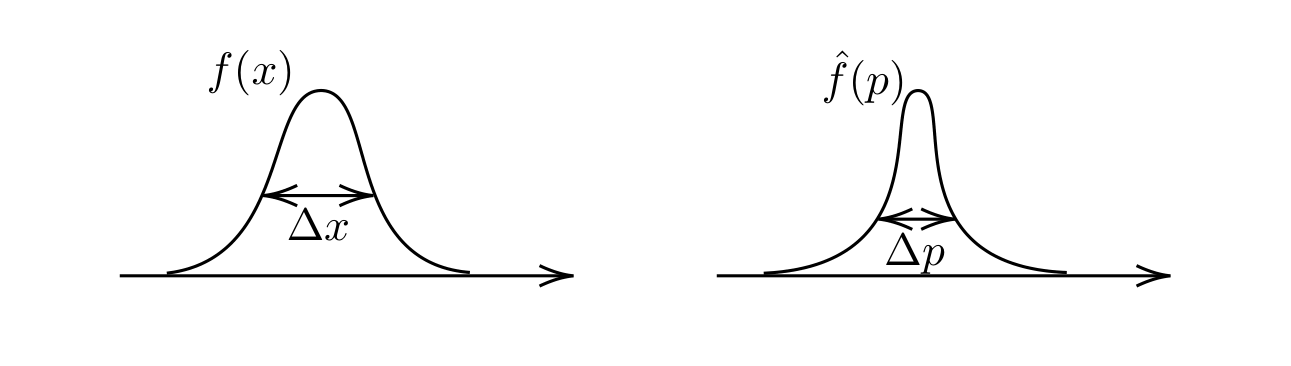
\includegraphics[width=0.62\textwidth]{figures/fig_p029_a.png}
\end{center}
% [图：原书 p.28，图内文字照原样保留；左为坐标空间中的 $f(x)$ 与其宽度 $\Delta x$，右为动量空间中的 $\hat f(p)$ 与其宽度 $\Delta p$，原图无题注]

\subsection{哈密顿算子}

我们考虑质量为 $m$ 的粒子在势 $V(\mathbf x,t)$ 中运动。经典地，动力学由相空间中的哈密顿函数 $\mathcal H(\mathbf x,\mathbf p)$ 描述：
\[
\mathcal H=\frac{\mathbf p^2}{2m}+V(\mathbf x,t).
\]
这里 $\frac{\mathbf p^2}{2m}$ 是动能，$V$ 是实值的势能。

量子力学中，哈密顿函数将被量子化为自伴的哈密顿算子。自然的候选是作替换
\[
x^i\to\hat x^i,\qquad p_i\to\hat p_i.
\]
如此得到哈密顿算子
\[
\hat H=-\frac{\hbar^2}{2m}\nabla^2+V(\mathbf x,t),
\]
其中 $\nabla^2=\sum_i\frac{\pa}{\pa x^i}\frac{\pa}{\pa x^i}$ 是拉普拉斯算子。

本章我们主要研究上述形式的哈密顿算子。相应的薛定谔方程现在取显式形式
\[
\ii\hbar\frac{\pa}{\pa t}\Psi(\mathbf x,t)
=\left(-\frac{\hbar^2}{2m}\nabla^2+V(\mathbf x,t)\right)\Psi(\mathbf x,t).
\]
哈密顿算子 $\hat H$ 是微分算子这一事实，还带来概率守恒的局部形式。令
\[
\rho(\mathbf x,t)=\abs{\Psi(\mathbf x,t)}^2
\]
% [原文 p.29]
为概率密度。如我们所见，薛定谔方程蕴含总概率守恒
\[
\frac{\rd}{\rd t}\int\rd^n\mathbf x\,\rho(\mathbf x,t)=0.
\]
这一守恒律可提升为标准局部形式
\[
\frac{\pa}{\pa t}\rho+\nabla\cdot\vec j=0,
\]
其中 $\vec j$ 是某个流向量场。的确，利用薛定谔方程与 $V$ 的实值性，
\[
\begin{aligned}
\frac{\pa}{\pa t}\rho
&=\frac{\pa\ol{\Psi}}{\pa t}\Psi+\ol{\Psi}\frac{\pa\Psi}{\pa t}\\
&=\frac{\ii}{\hbar}\bigl(\overline{\hat H\Psi}\bigr)\Psi-\frac{\ii}{\hbar}\ol{\Psi}\bigl(\hat H\Psi\bigr)\\
&=\frac{\ii}{\hbar}\left[-\frac{\hbar^2}{2m}(\nabla^2\ol{\Psi})\Psi
+V\ol{\Psi}\Psi+\frac{\hbar^2}{2m}\ol{\Psi}\nabla^2\Psi-V\ol{\Psi}\Psi\right]\\
&=-\frac{\ii\hbar}{2m}\nabla\cdot\bigl[(\nabla\ol{\Psi})\Psi-\ol{\Psi}\nabla\Psi\bigr],
\end{aligned}
\]
\[
\Longrightarrow\quad
\vec j=\frac{\ii\hbar}{2m}\bigl[(\nabla\ol{\Psi})\Psi-\ol{\Psi}\nabla\Psi\bigr]
=\frac{\hbar}{m}\Imag\bigl(\ol{\Psi}\nabla\Psi\bigr).
\]
这里 $\nabla=(\pa_{x_1},\cdots,\pa_{x_n})$ 是梯度算子。于是
\[
\vec j=\frac{\hbar}{m}\Imag\bigl(\ol{\Psi}\nabla\Psi\bigr),
\]
称为\emph{概率流}。对任意固定区域 $V\subset\R^n$，有
\[
\frac{\rd}{\rd t}\int_V\rd^n\mathbf x\,\rho(\mathbf x,t)
=\int_V\rd^n\mathbf x\,\pa_t\rho
=-\int_V\rd^n\mathbf x\,\nabla\cdot\vec j
=-\int_{\partial V}\rd\vec\sigma\cdot\vec j.
\]
这里 $\rd\vec\sigma$ 是 $\partial V$ 上的向量面积元。它说的是：在 $V$ 内找到粒子的概率，其变化率等于概率流经边界 $\partial V$ 流出的通量。

\subsection{定态}

我们考虑量子粒子在只依赖位置 $\mathbf x\in\R^n$、不依赖时间的势 $V=V(\mathbf x)$ 中运动。此时哈密顿算子 $\hat H$ 不依赖时间
\[
\hat H=-\frac{\hbar^2}{2m}\nabla^2+V(\mathbf x).
\]
我们寻找薛定谔方程如下形状的特解
\[
\Psi(\mathbf x,t)=\ee^{-\ii\omega t}\psi(\mathbf x).
\]
把它代入薛定谔方程，得到
\[
\hat H\psi(\mathbf x)=E\psi(\mathbf x) \tag{$*$}
\]
其中 $E=\hbar\omega$。换言之，$\psi(\mathbf x)$ 是哈密顿算子 $\hat H$ 的本征态。基于我们对测量的讨论，本征值 $E$ 自然被理解为该态 $\psi$ 的能量。

% [§1.5 的 \takeaway 已移至 ch01b.tex（本节的最后一段在原书 p.30，属下一块）]

% [块界：本块止于 PDF p.30（原书 p.29）末句“……该态 $\psi$ 的能量。”；下一块 ch01b 从 “Equation (*) is called the time-independent Schrödinger equation.” 续起，不要重复本句。]

